% Chapter Template

\chapter{RISC-V KeyStone} % Main chapter title

\label{Chapter4} % Change X to a consecutive number; for referencing this chapter elsewhere, use \ref{ChapterX}

\section{Introduction}
Keystone基于RISCV指令集架构,是第一个构建定制TEE的开源框架。Keystone使用了基于硬件的简单抽象,如内存隔离和在不可信部件(如OS)之下的可编程层。Keystone从这些抽象中构建可重用的TEE核心原语,同时允许特定于平台的修改和应用程序特性。

\section{威胁模型}
Keystone信任以下部分:
\begin{itemize}
	\item [1)]
	PMP (Physical Memory Protection)
	\item [2)]
	信任RISC-V架构无BUG
	\item [3)]
	Keystone用户只在Secure Monitor被验证后信任它
	\item [4)]
	Secure Monitor只信任硬件
	\item [5)]
	Root of Trust信任Secure Monitor
	\item [6)]
	Enclave app信任Secure Monitor和Root of Trust
\end{itemize}
Keystone假设有以下这些攻击者:
\begin{itemize}
	\item [1)]
	物理攻击者可以截获、修改或重放离开chip package的信号。Keystone假设物理攻击者不会影响chip package内的组件。
	\item [2)]
	软件攻击者可以控制主机应用程序、不受信任的操作系统、网络通信、启动恶意的enclave、任意修改任何未受TEE保护的内存,以及添加/删除/重放enclave消息。
	\item [3)]
	侧通道攻击者通过cache side-channel、timing side-channel或control channel被动地观察可信组件和不可信组件之间的交互,从而收集信息。
	\item [4)]	
	拒绝服务攻击者可以攻击enclave或主机OS。Keystone不防御这些攻击,因为OS可以在任何时候拒绝为用户应用程序提供服务。
\end{itemize}

\section{保证的安全性质和能够防御的一些具体攻击}
\subsection{安全保证}
\paragraph{内存隔离}
Keystone使用RISC-V架构提供的PMP (Physical Memory Protection) 来进行内存保护。
PMP通过定义相应的PMP region来限制User-mode和Supervisor-mode的内存访问。
RISC-V架构拥有16个pmpaddr寄存器和4个pmpcfg寄存器,pmpaddr寄存器用来存放相应region的地址(物理地址),
pmpcfg寄存器用来定义访存权限、region区间对齐方式以及是否锁定该region.
\paragraph{通过Secure Monitor加强内存隔离}
在RISC-V架构中,存在Machine-mode这一高于Supervisor-mode的特权级,Secure Monitor便运行在这一模式。
在CPU将控制转移给enclave时,Secure Monitor会enable当前要执行的enclave的PMP permission bits. 
并disable OS拥有的所有PMP的permission bits,以此来保证enclave只能访问自己的region.
在CPU从enclave退出时,Secure Monitor会disable enclave的PMP permission bits,
并enable OS的PMP permission bits.
Secure Monitor的这些操作,在更高的权限级(M-mode)保证了PMP的安全性。

\subsection{能够预防的具体攻击}
对于Enclave的保护:
\begin{itemize}
	\item [1)]
	\textbf{Mapping Attacks} Enclave运行在可信的RT(runtime)之上,故RT本身不会去做恶意的mapping. 并且OS给enclave配的页表会经过SM的检查。
	\item [2)]
	\textbf{Syscall Tampering Attaks} Enclave调用syscall可能会受到Syscall Tampering Attack,Keystone可以将已有的防御措施(如SCONE、Graphene等)作为Plugin来防御这些攻击。
	\item [3)]
	\textbf{Side-channel Attacks} Keystone提供cache partitioning,可以防止Side-channel Attacks.
\end{itemize}

\section{性能、可扩展性(scalability)、灵活性等分析}
\subsection{性能}
\begin{figure}[]
    \centering
    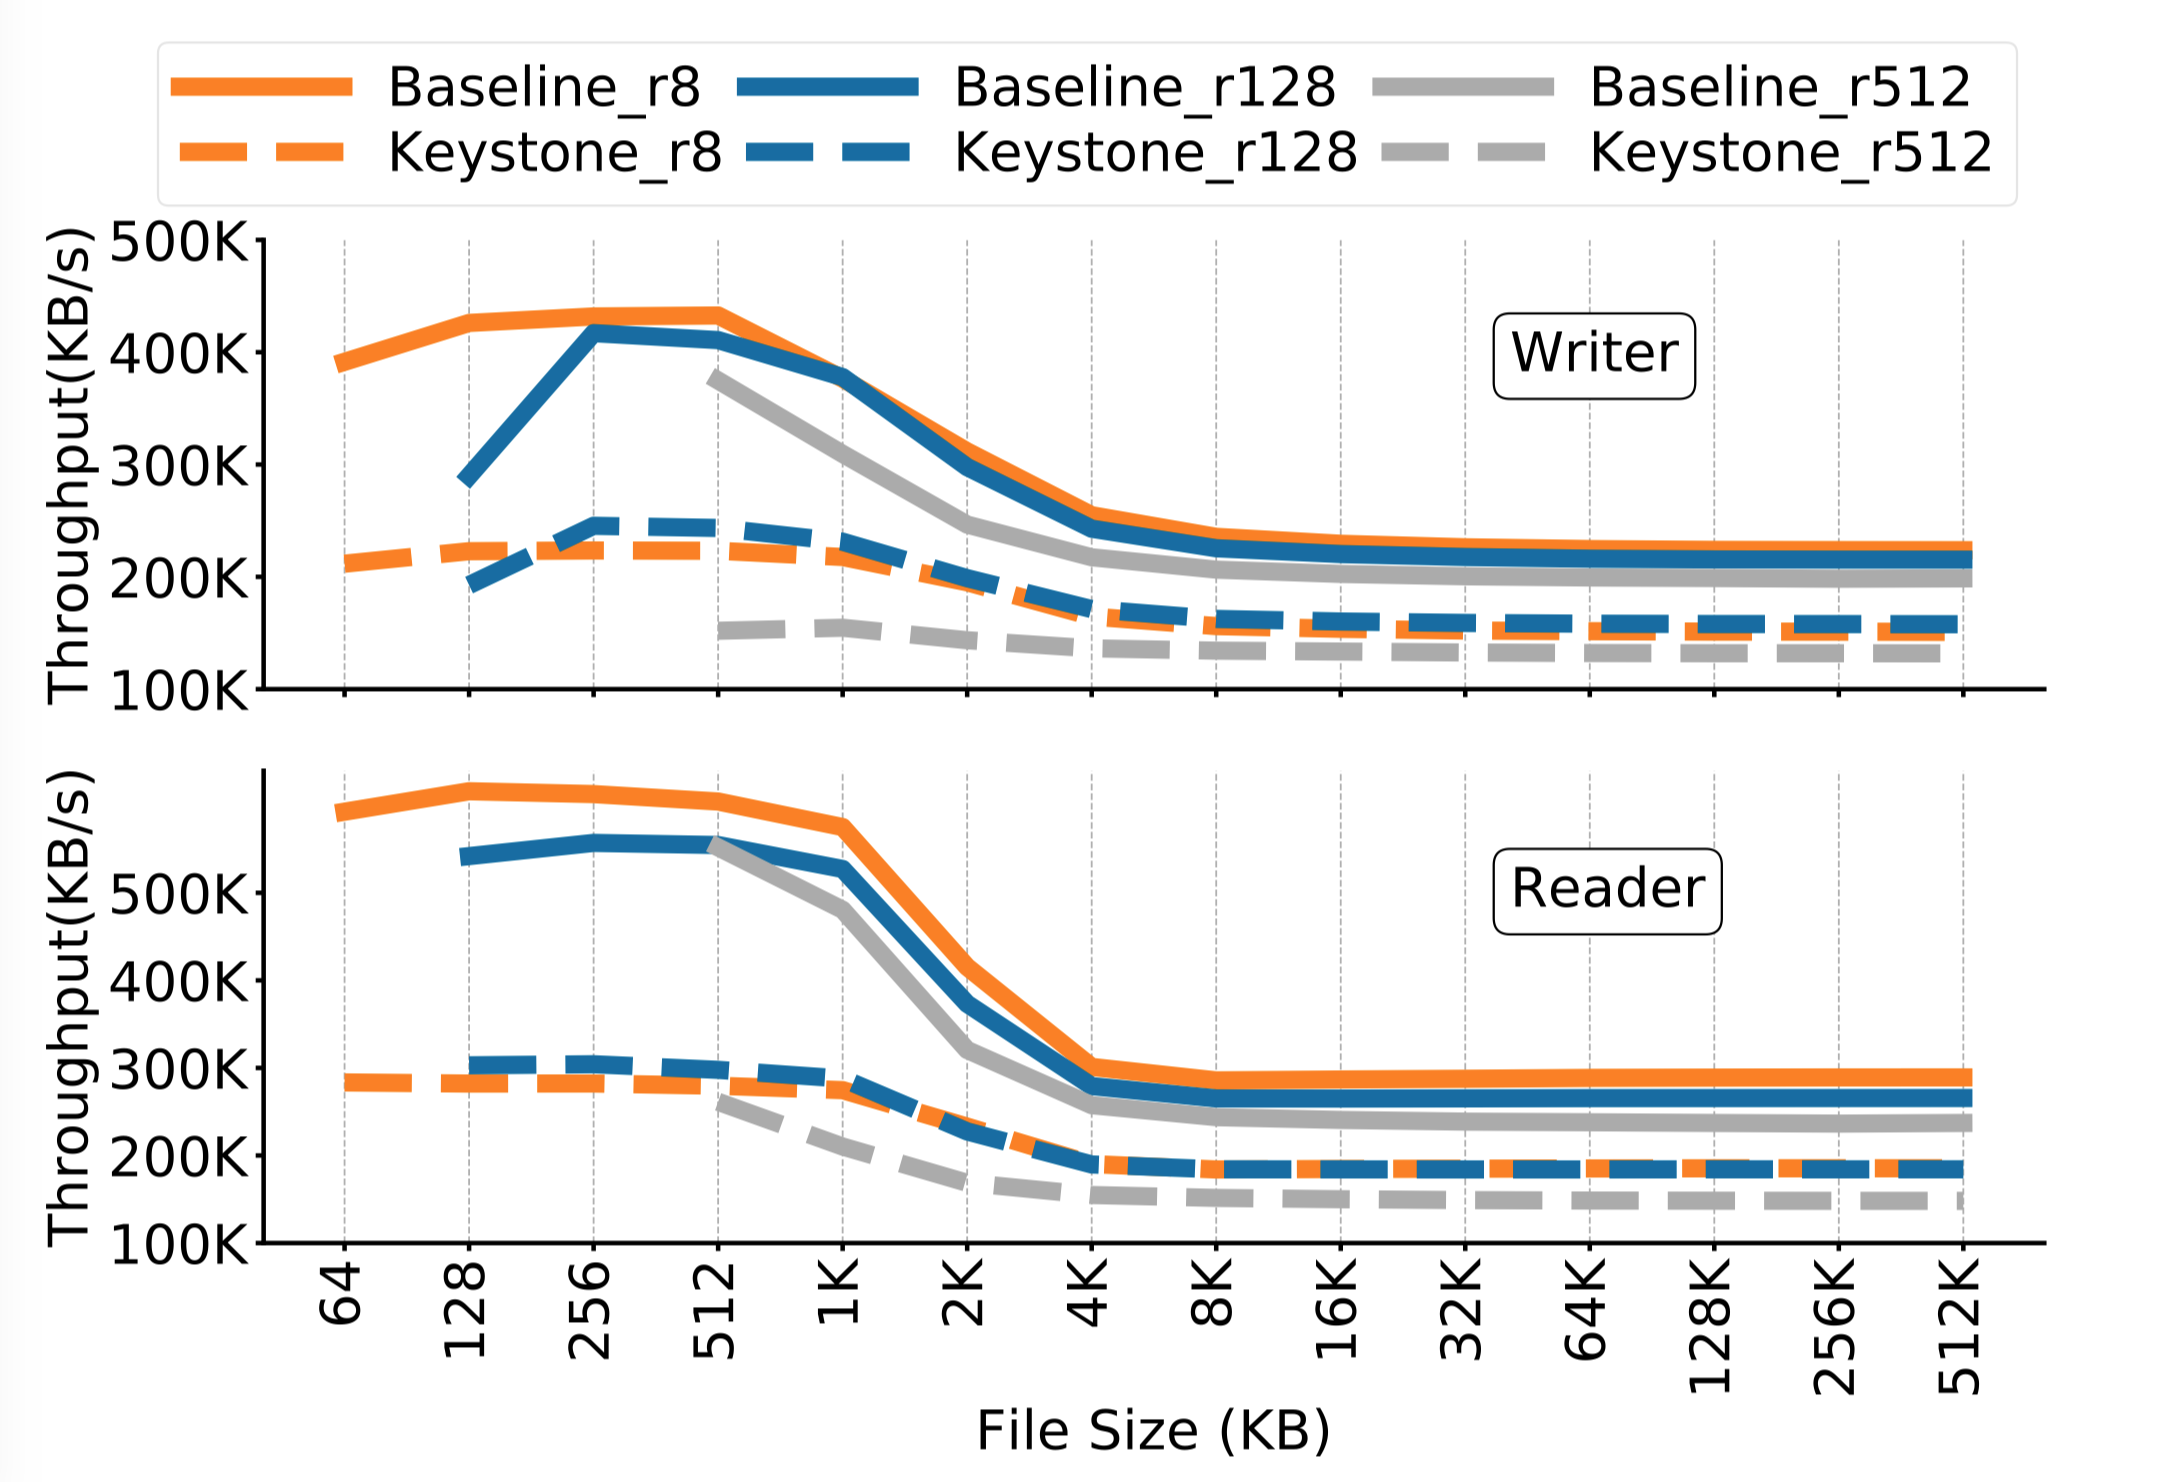
\includegraphics[width=1\textwidth]{memory-eval.png}    
    \caption{Keystone和baseline运行IOZone benchmark}
\end{figure}
上图是Keystone和baseline(linux)运行RV8 benchmark,可以看到,Keystone的访存性能大概在baseline的一半左右,考虑到其运行在enclave内,这个overhead还能接受。
\begin{figure}[]
    \centering
    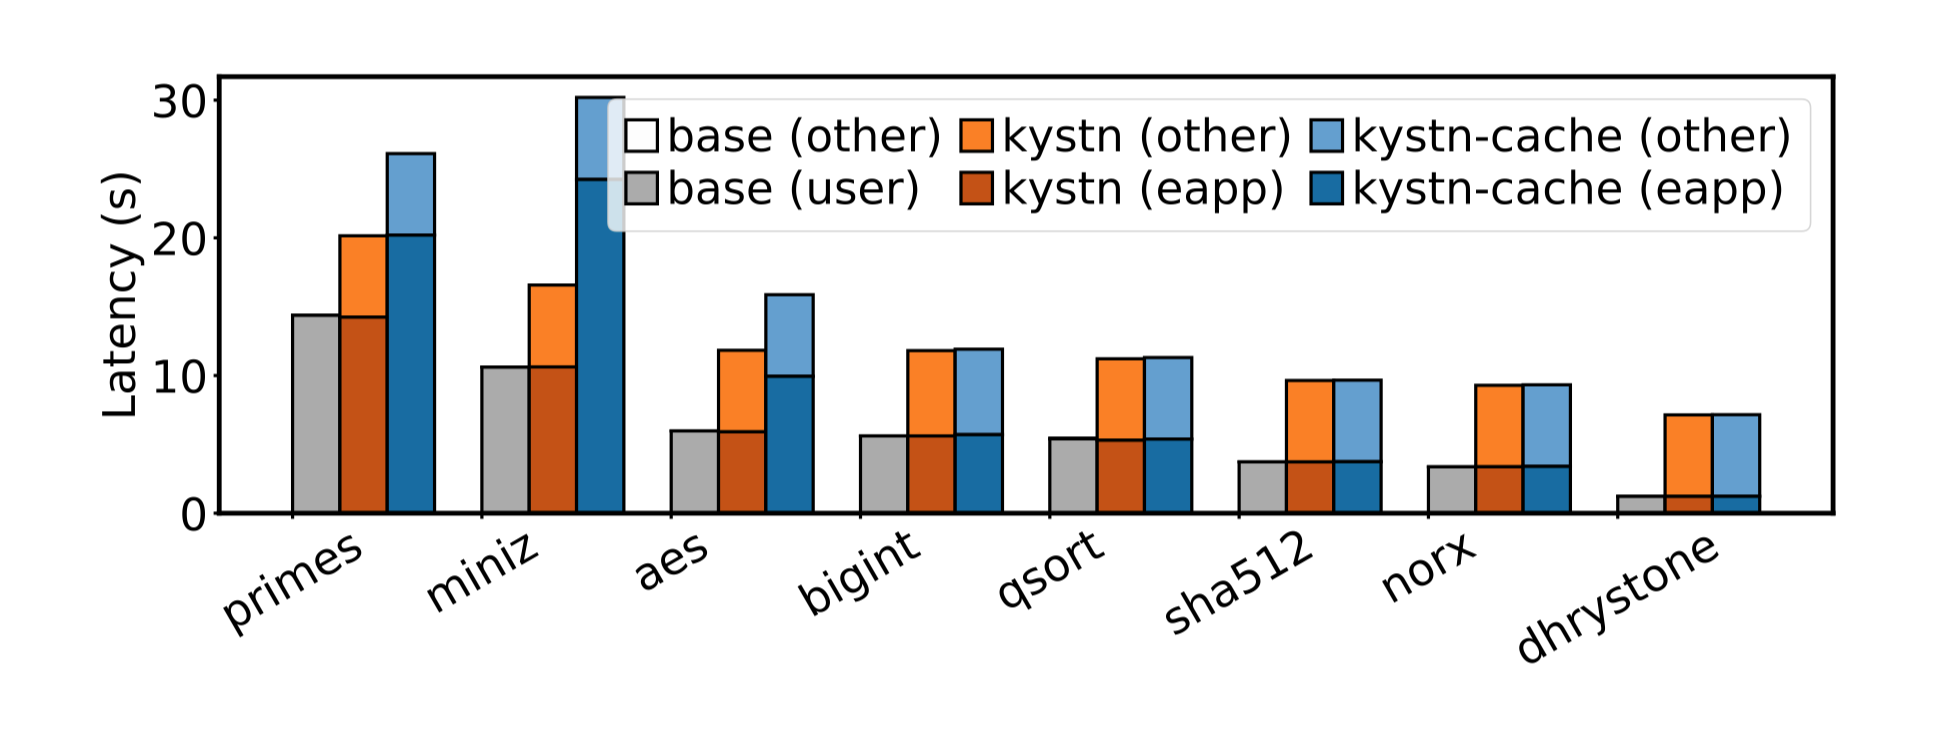
\includegraphics[width=1\textwidth]{calculation-eval.png}    
    \caption{Keystone和baseline运行RV8 benchmark}
\end{figure}
上图是Keystone和baseline(linux)运行IOZone benchmark,可以看到,由于workload本身在enclave内,Keystone并没有增加计算的latency.
\subsection{可扩展性和灵活性}
由于Keystone是基于RISC-V的开源框架,所以其可扩展性和灵活性都颇佳。
首先,由于RISC-V架构非常轻便,开发者可以很方便的自己修改硬件特性,Keystone可以部署在支持RISC-V架构的平台上。
其次,使用PMP做内存隔离非常灵活。在RISC-V里一共有16个PMP寄存器,可以灵活的给多个enclave分配region。不会像SGX那样,对EPC的大小有限制,也不要求一个enclave的物理地址空间必须要连续。
最后,Keystone支持自定义的Plugin选择,可以让开发者自由选择需要的安全特性,使其可扩展性和灵活性更上一个台阶。

\section{不足}
\begin{itemize}
	\item [1)]
	Keystone PMP寄存器的数量只有16个,
	还要分配一部分来保护Secure Monitor以及供OS正常访存使用。
	这样一来,可以用来给enclave使用的PMP寄存器就更少了。
	\item [2)]
	Keystone不能防御DoS攻击,因为其还是需要一个正常运行的OS(配页表、syscall等),恶意的OS可以拒绝服务用户。而Keystone没有修改OS,所以不能防御DoS攻击。
\end{itemize}

\section{本章小结}
本章从Keystone的威胁模型出发,详细介绍了其提供的安全保障。
并且举例介绍了keystone可以防御的具体攻击。
本章其后分析了keystone的性能,并且就其可扩展性与灵活性做了分析。
最后,本章简述了keystone的不足之处。
